\section{Решение двумерной начально-краевой задачи для дифференциальных уравнений в частных производных параболического типа}

\subsection{Постановка задачи}
Используя схемы переменных направлений и дробных шагов, решить двумерную начально-краевую задачу для дифференциального уравнения параболического типа. В различные моменты времени вычислить погрешность численного решения путем сравнения результатов с приведенным в задании аналитическим решением $U(x, t)$. Исследовать зависимость погрешности от сеточных параметров $\tau$, $h_x$, $h_y$.

{\bfseries Вариант:} 8
\begin{align*} 
& \frac{\partial u}{\partial t} = a \frac{\partial^2 u}{\partial x^2} + b \frac{\partial^2 u}{\partial y^2} + \sin x \sin y (\mu \cos(\mu t) + (a + b) \sin(\mu t)) \\
& u(0, y, t) = 0 \\
& u(2 \pi, y, t) = \sin y \sin(\mu t) \\
& u(x, 0, t) = 0 \\
& u(x, 2 \pi, t) = \sin x \sin(\mu t)\\
& u(x, y, 0) = 0 \\
& U(x, y) = \sin x \sin y \sin(\mu t) \\
& a = 1,\ b = 1,\ \mu = 1 \\
\end{align*}

\pagebreak

\subsection{Результаты работы}
\begin{figure}[h!]
\centering
\subfigure[]{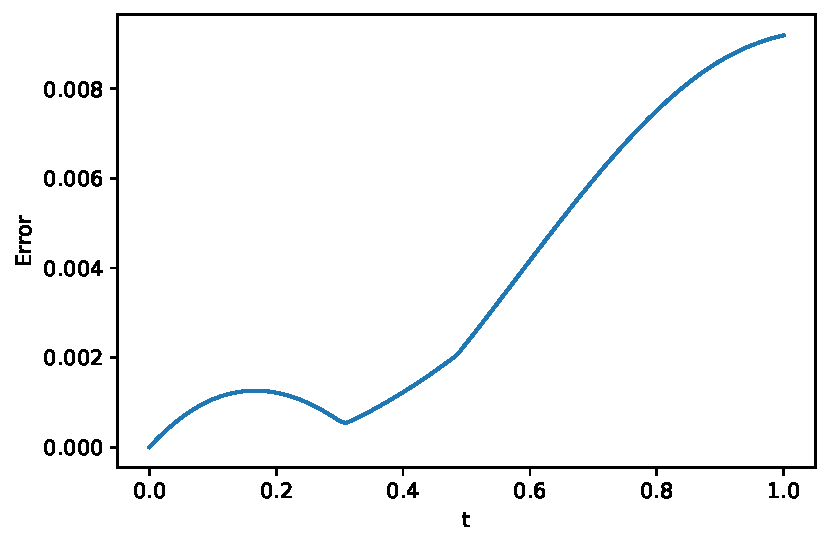
\includegraphics[width=.5\textwidth]{lab8_adm_error_plot}}\hfill
\subfigure[]{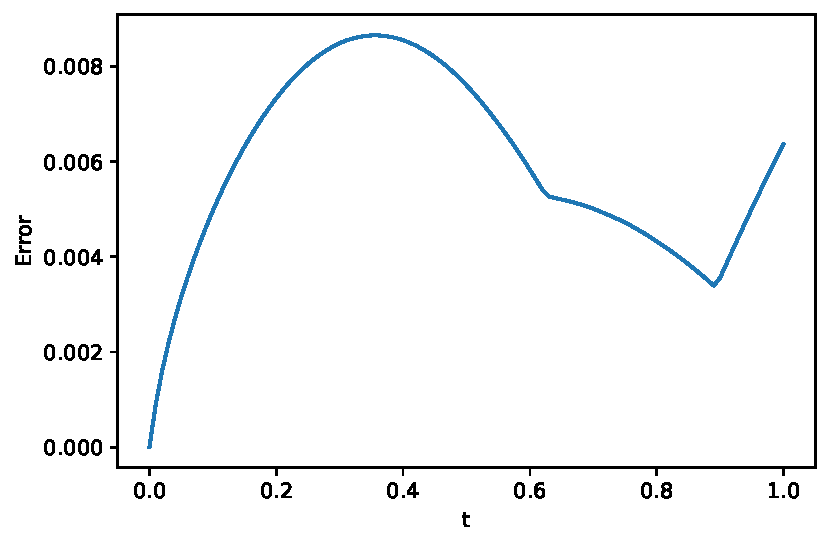
\includegraphics[width=.5\textwidth]{lab8_fsm_error_plot}}
\caption{Максимум погрешности решения в зависимости от времени для (a) метода переменных направлений и (b) метода дробных шагов}
\end{figure}

\vspace{24pt}

\begin{figure}[h!]
\centering
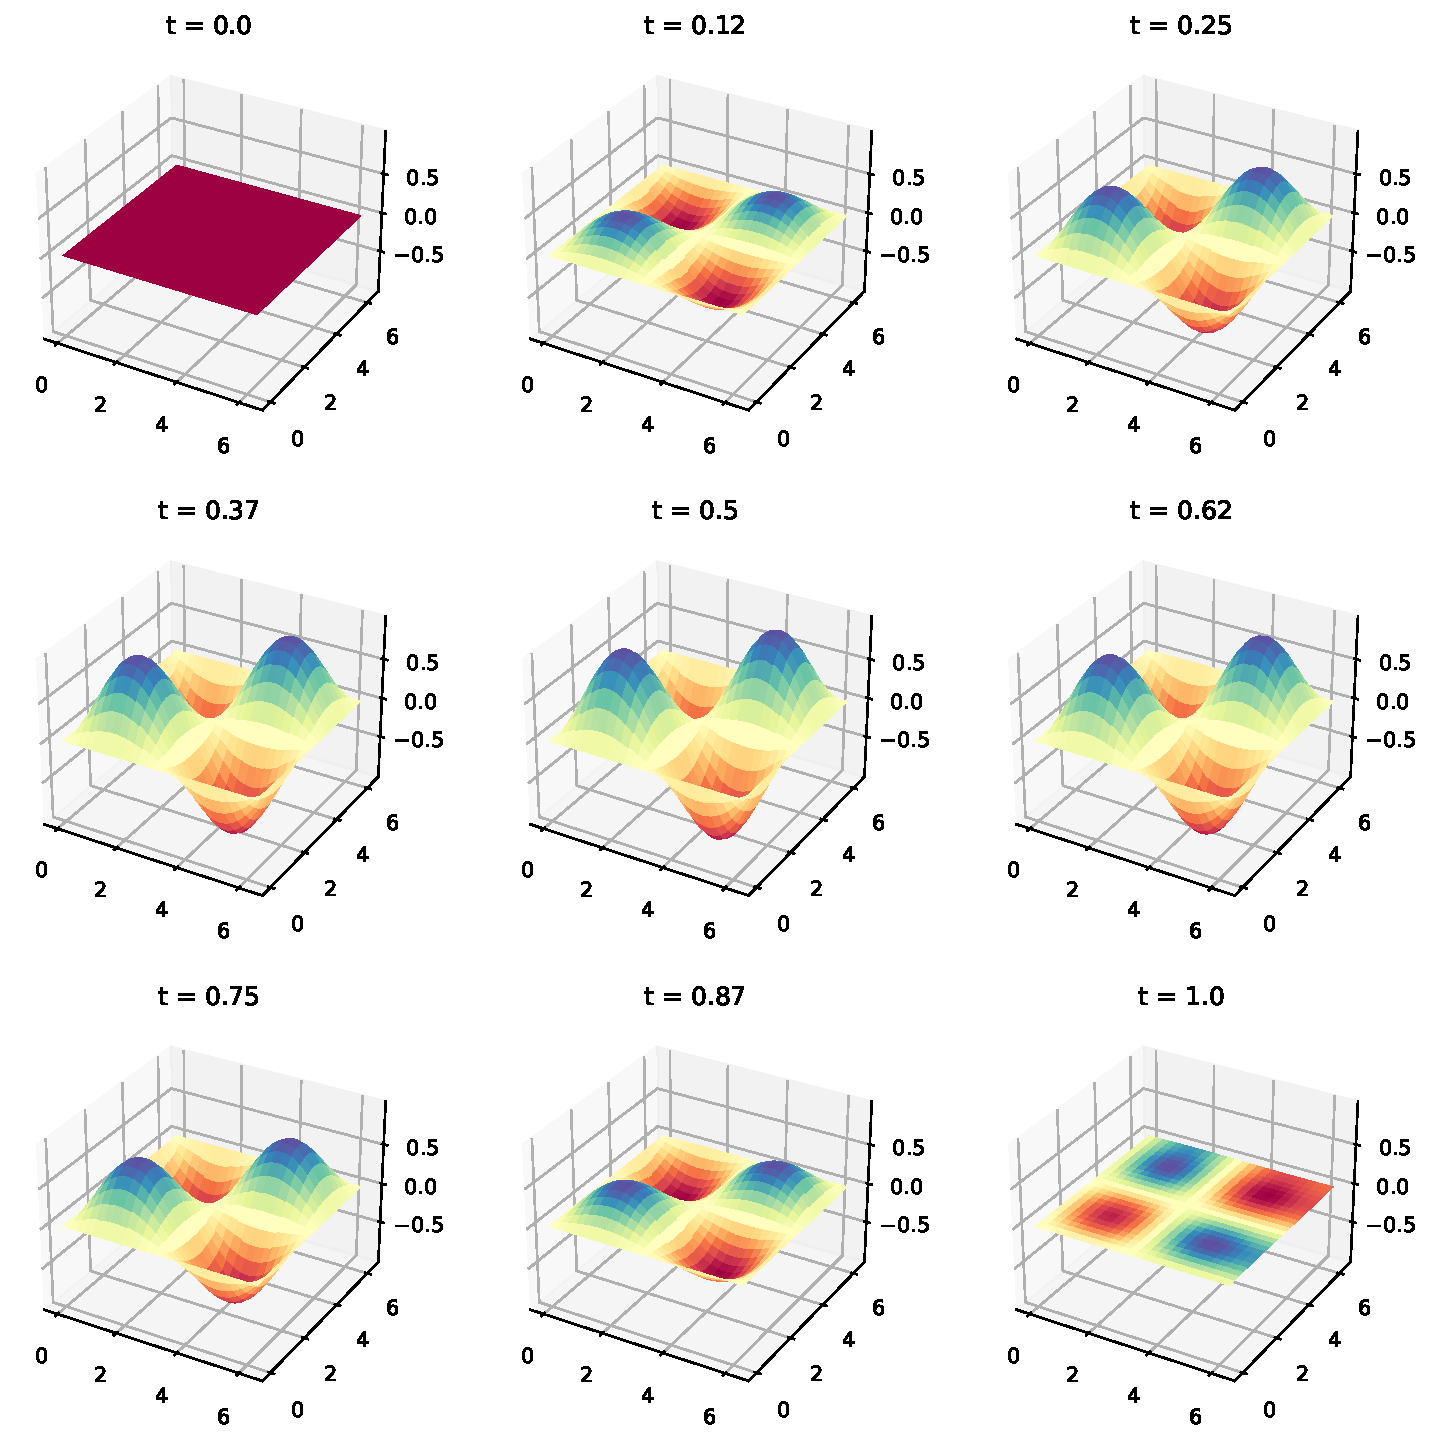
\includegraphics[width=.48\textwidth]{lab8_adm_solution}\hfill
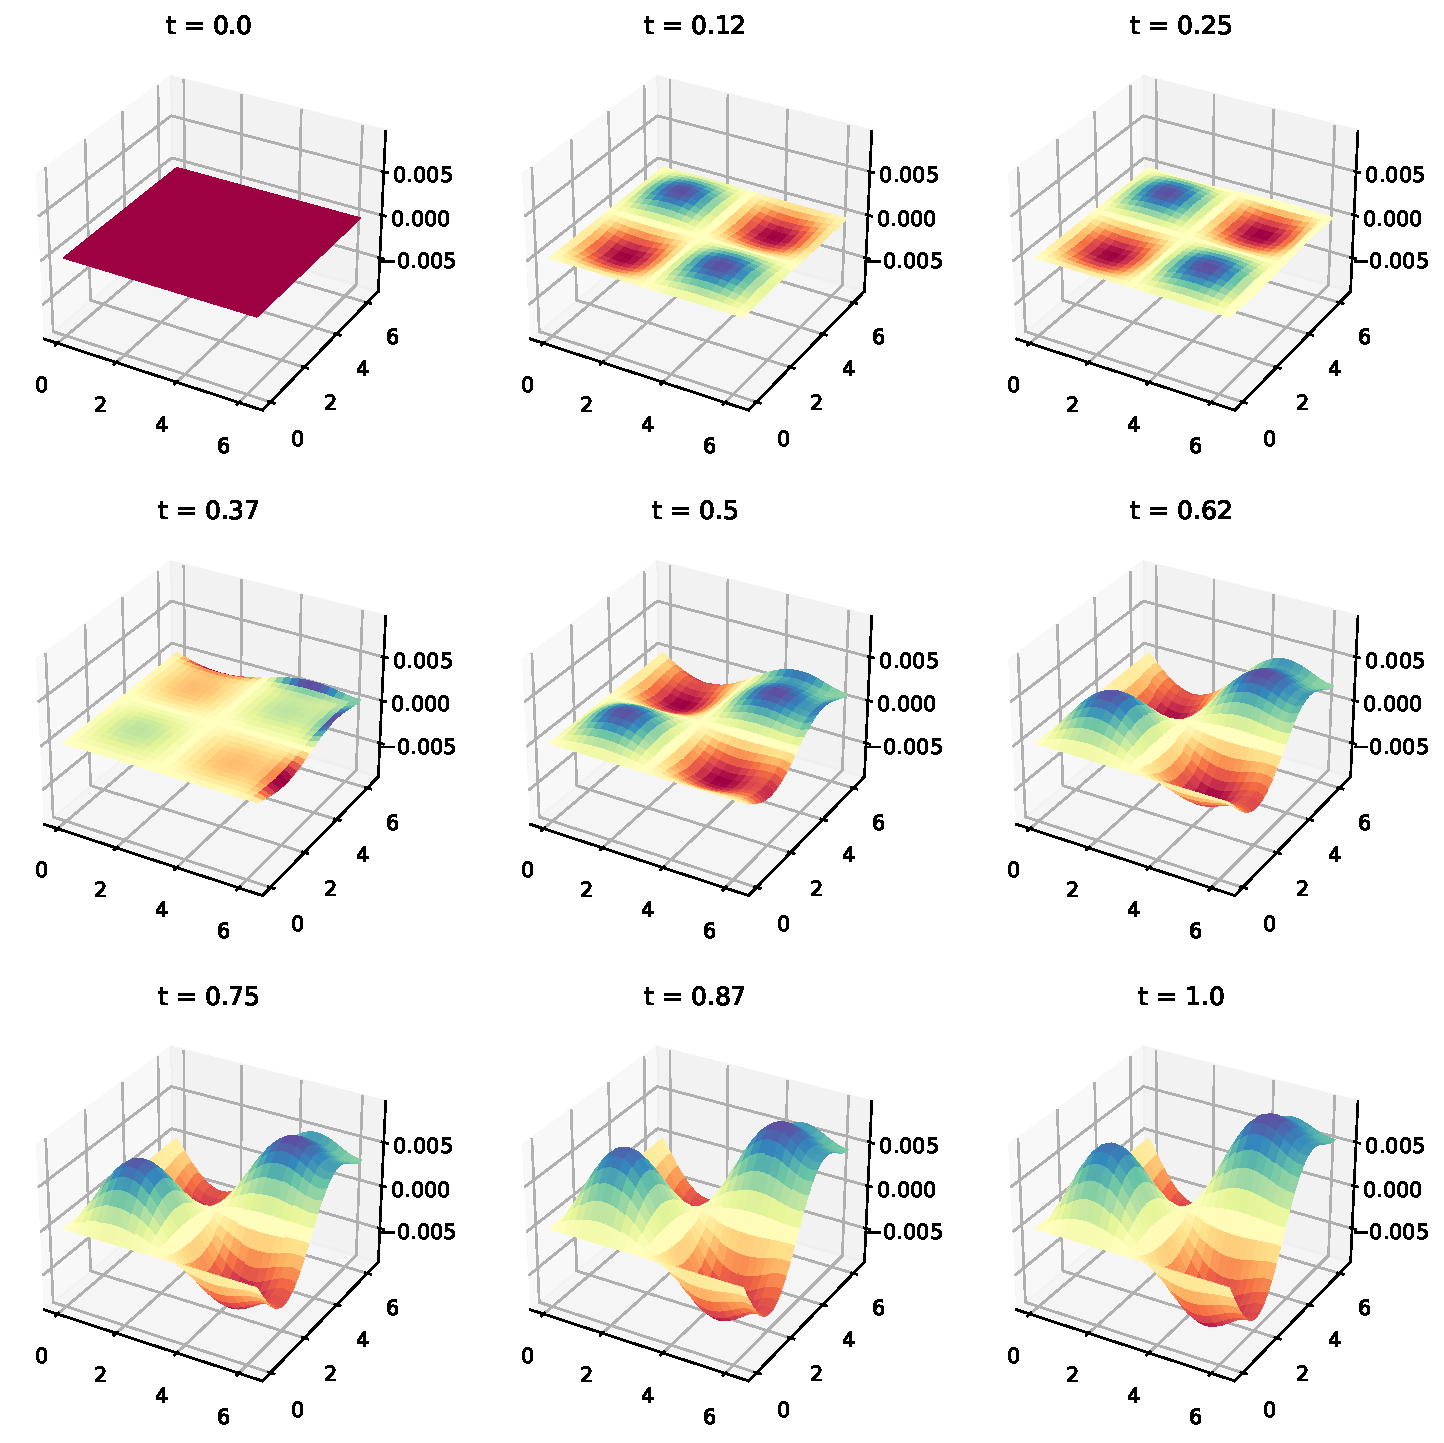
\includegraphics[width=.48\textwidth]{lab8_adm_error}
\caption{Эволюция решения и погрешности для метода переменных направлений}
\end{figure}

\pagebreak

\begin{figure}[h!]
\centering
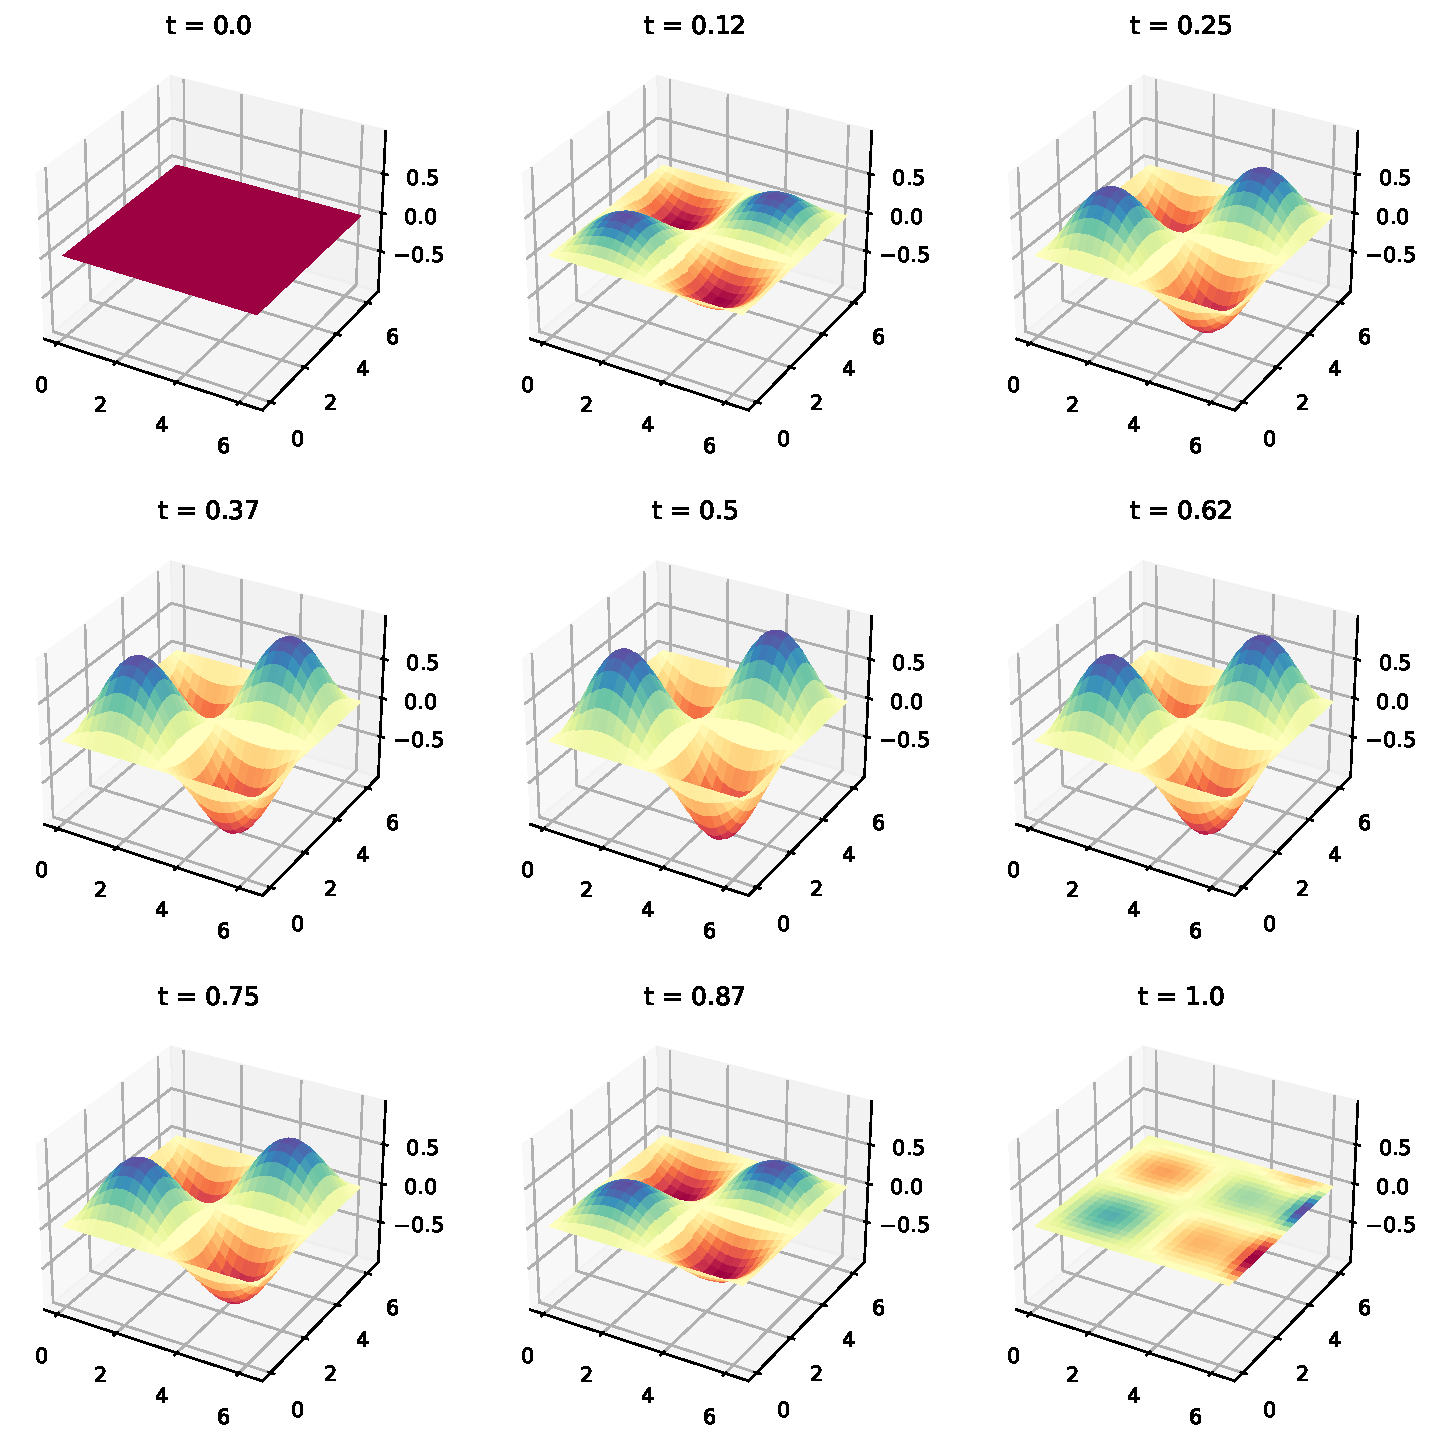
\includegraphics[width=.48\textwidth]{lab8_fsm_solution}\hfill
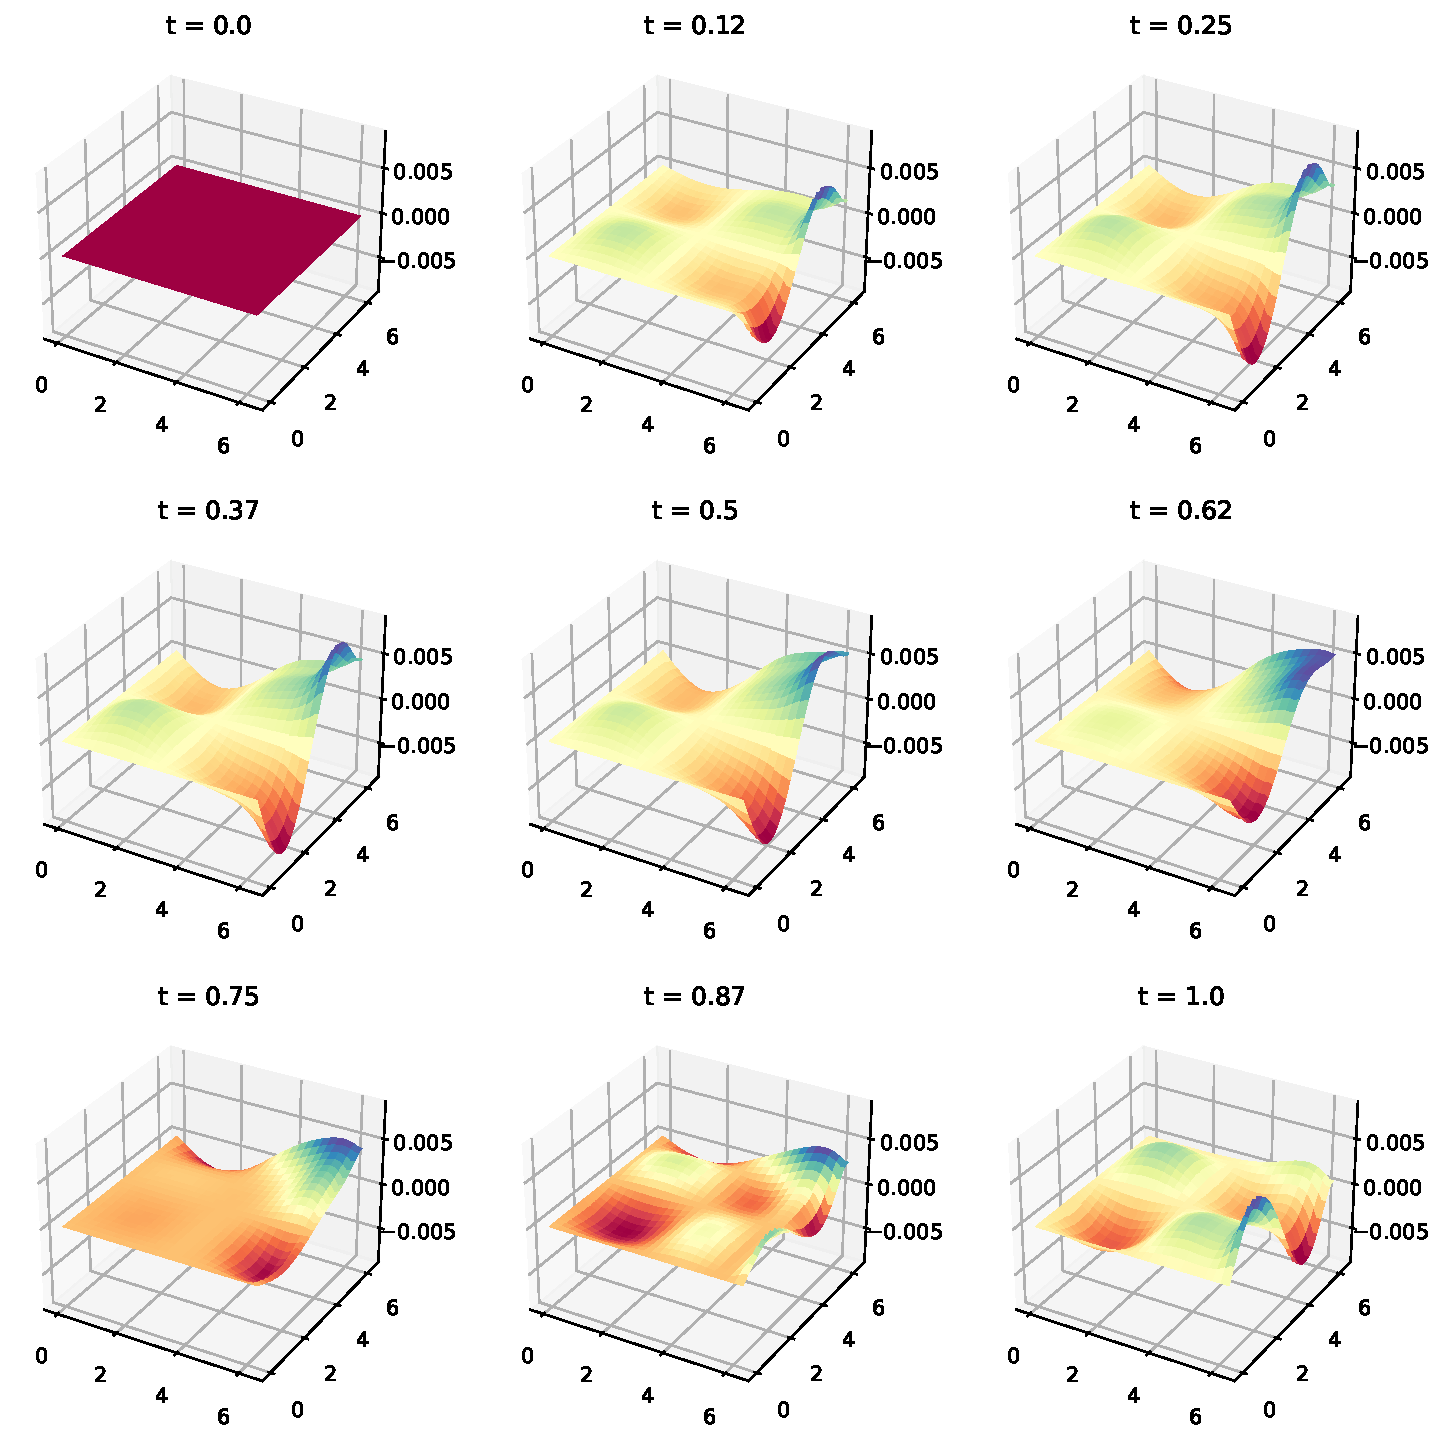
\includegraphics[width=.48\textwidth]{lab8_fsm_error}
\caption{Эволюция решения и погрешности для метода дробных шагов}
\end{figure}

\subsection{Исходный код}
\lstinputlisting{../../include/partial_differential/parabolic2d_pde.hpp}
\pagebreak
